\documentclass[a4, 11pt, titlepage]{article}

\usepackage[french]{babel}
\usepackage{fontspec}
\setmainfont{EB Garamond}[Numbers={Proportional, OldStyle},
RawFeature={+ss06}, ItalicFeatures={Ligatures=Rare}]
\usepackage{hyperref}
\usepackage{amsmath}
\usepackage{amssymb}
\usepackage{verbatim}

\usepackage{float}

\usepackage{epigraph}

\usepackage{url}

\usepackage{graphicx}


% prettier greek letters
\renewcommand{\phi}{\varphi}
\renewcommand{\epsilon}{\varepsilon}

% sets
\newcommand{\N}[0]{\mathbb{N}}
\newcommand{\Z}[0]{\mathbb{Z}}
\newcommand{\Q}[0]{\mathbb{Q}}
\newcommand{\R}[0]{\mathbb{R}}

\newcommand{\qed}[0]{\begin{flushright} $\Box$ \end{flushright}}

\newcommand{\ie}[0]{\textit{i.e.}}

% relation symbols
\newcommand{\rel}[0]{\mathcal{R}}

% calligraphic letters
\newcommand{\Mc}[0]{\mathcal{M}}
\newcommand{\Nc}[0]{\mathcal{N}}
\newcommand{\Lc}[0]{\mathcal{L}}
\newcommand{\Uc}[0]{\mathcal{U}}
\newcommand{\Pc}[0]{\mathcal{P}}

\newcommand{\fouine}[0]{\texttt{fouine}}

\setlength{\epigraphwidth}{0.6\textwidth}

\title{Rapport projet Fouine}
\author{Robin \bsc{Jourde} \& Nicolas \bsc{Nardino}}
\date{mai 2021}

\begin{document}

\maketitle

\begin{center}
  \small
  \verbatiminput{fouine-ascii.txt}
\end{center}

\newpage

\epigraph{
À l'origine fut la vitesse, la pure programmation fonctionnelle, le
<<~$\lambda x.e$~>>

Puis l'évaluation décéléra, prit consistance et forme, jusqu'aux lenteurs
habitables, jusqu'au \texttt{let}, jusqu'à vous.

Bienvenue à toi, lente fouine liée, poussif tresseur de fonctions
récursives.}{\cite{LaHorde}}




\tableofcontents

\section{Présentation}

Foino (Martes foina) aŭ estas specio de marteso kiu havas brilan
blugrizan ĝis blubrunan hararon, iom malpli delikatan ol tiu de la
arbara marteso; duobla makulo sur la gorĝo estas blanka.~\cite{wiki:001}

\fouine\ est un interpréteur de \texttt{FouineJN} (Fouine
Joviale et Naturelle~\footnote{[Citation~Needed]}), sous-ensemble du
langage de programmation national, \textsc{OCaml}.

\fouine\ est programmé principalement \textsc{OCaml}~\ref{fig:ocaml},
et le parser associé est généré avec \textsc{Menhir}~\ref{fig:menhir}.

\begin{figure}[H]
  \centering
  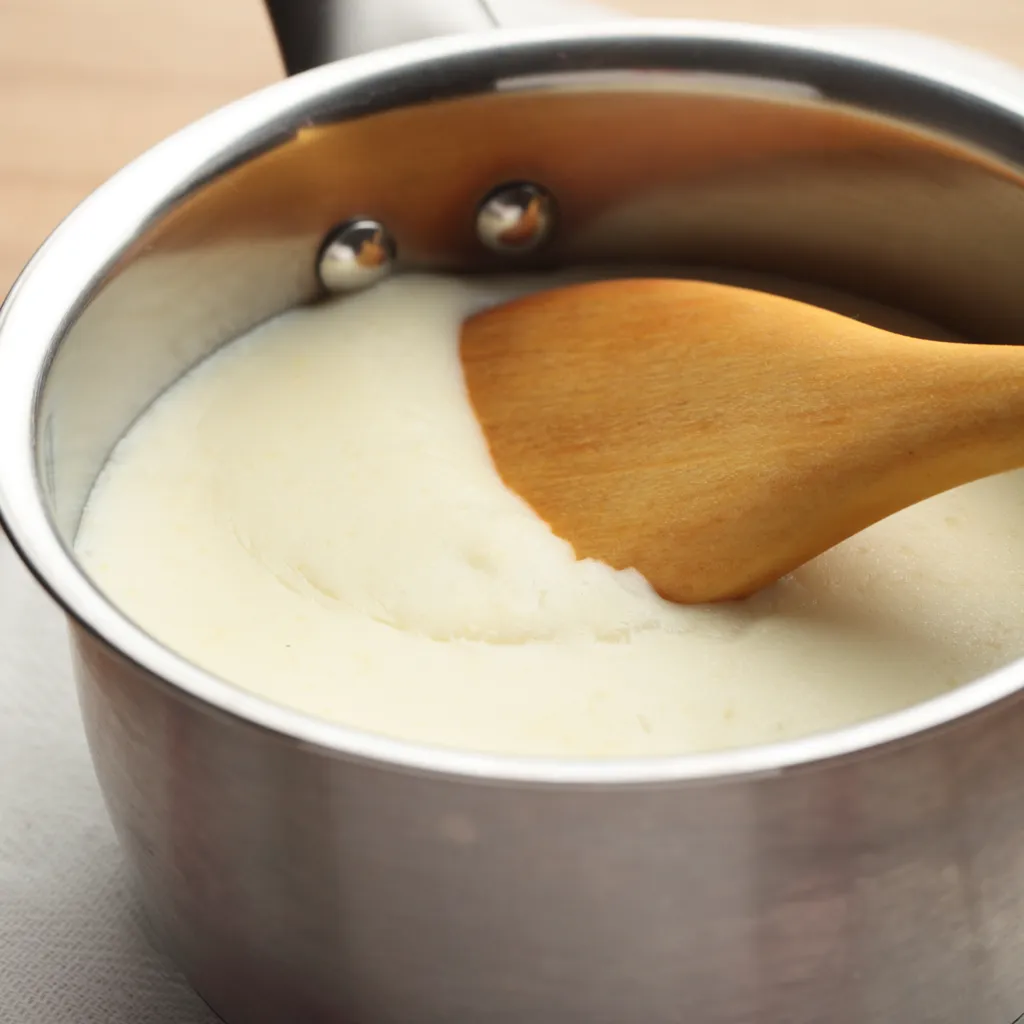
\includegraphics[width=0.33\linewidth]{figures/bechamel.png}
  \caption{\label{fig:ocaml} Exemple de béchamel, dans laquelle on
    peut trouver \texttt{caml}}
\end{figure}

\begin{figure}[H]
  \centering
  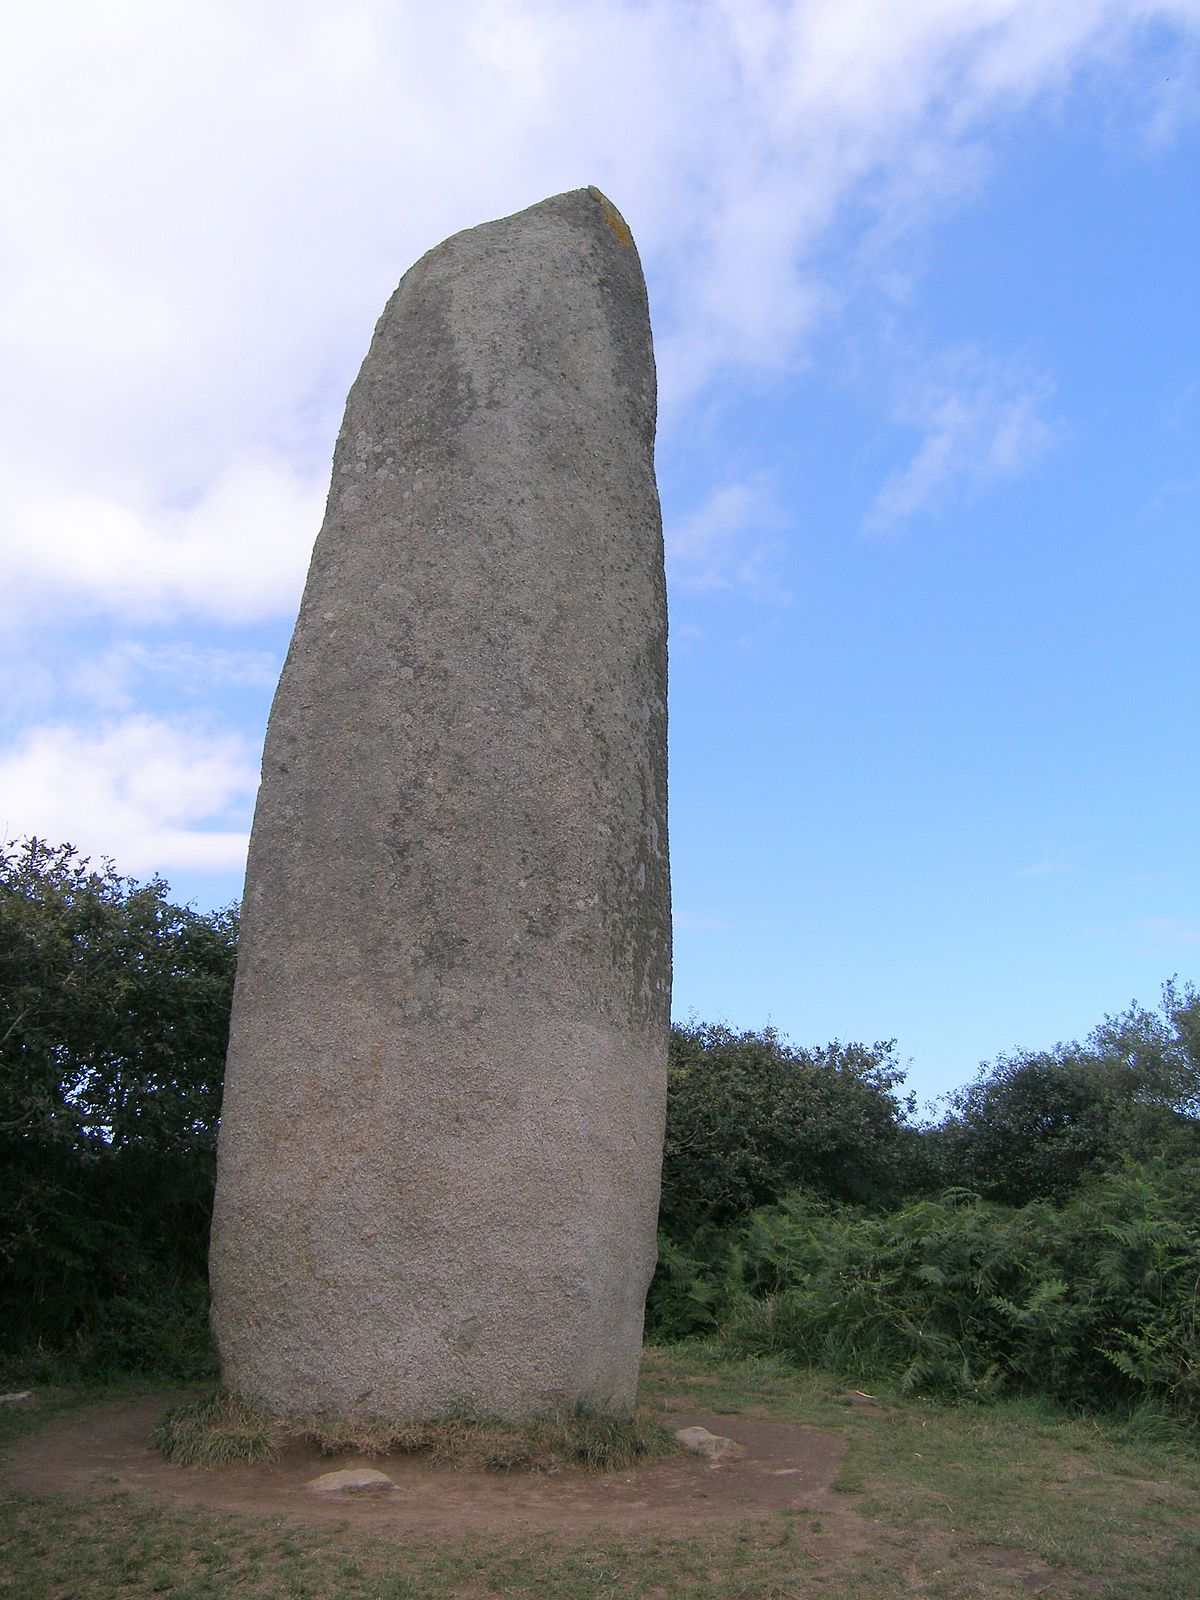
\includegraphics[width=0.33\linewidth]{figures/menhir.JPEG}
  \caption{\label{fig:menhir} Exemple de menhir}
\end{figure}


\cite{Landin66}.



\bsc{Tchana2025}~\cite{Tchana21}


\bibliographystyle{alpha}
\bibliography{biblio}

\end{document}
